%%% LaTeX Template: Article/Thesis/etc. with colored headings and special fonts
%%%
%%% Source: http://www.howtotex.com/
%%% Feel free to distribute this template, but please keep to referal to http://www.howtotex.com/ here.
%%% February 2011
%%%
%%% Modified May 2018 by CDM

%%%  Preamble
\documentclass[11pt,letterpaper]{article}
\usepackage[margin=1.0in]{geometry}
\usepackage[T1]{fontenc}
\usepackage[bitstream-charter]{mathdesign}
\usepackage[latin1]{inputenc}					
\usepackage{amsmath}						
\usepackage{xcolor}
\usepackage{cite}
\usepackage{hyphenat}
\usepackage{graphicx}
\usepackage{float}
\usepackage{subfigure}
\usepackage{sectsty}
\usepackage[compact]{titlesec} 
\usepackage[tablegrid]{vhistory}
\allsectionsfont{\color{accentcolor}\scshape\selectfont}

%%% Definitions
\definecolor{accentcolor}{rgb}{0.0,0.0,0.5} 
\newcommand{\teamname}{Resonance}
\newcommand{\productname}{Project LTunes}
\newcommand{\coursename}{CSE 4316: Senior Design I}
\newcommand{\semester}{Fall 2019}
\newcommand{\docname}{System Requirements Specification}
\newcommand{\department}{Department of Computer Science \& Engineering}
\newcommand{\university}{The University of Texas at Arlington}
\newcommand{\authors}{Amir Dhungana \\ Anish Yonjan \\ Nikhil Purohit \\ Rabinson Shrestha \\ Raul Jimenez \\ Roberto Torres}

%%% Headers and footers
\usepackage{fancyhdr}
	\pagestyle{fancy}						% Enabling the custom headers/footers
\usepackage{lastpage}	
	% Header (empty)
	\lhead{}
	\chead{}
	\rhead{}
	% Footer
	\lfoot{\footnotesize \teamname \ - \semester}
	\cfoot{}
	\rfoot{\footnotesize page \thepage\ of \pageref{LastPage}}	% "Page 1 of 2"
	\renewcommand{\headrulewidth}{0.0pt}
	\renewcommand{\footrulewidth}{0.4pt}

%%% Change the abstract environment
\usepackage[runin]{abstract}			% runin option for a run-in title
%\setlength\absleftindent{30pt}			% left margin
%\setlength\absrightindent{30pt}		% right margin
\abslabeldelim{\quad}	
\setlength{\abstitleskip}{-10pt}
\renewcommand{\abstractname}{}
\renewcommand{\abstracttextfont}{\color{accentcolor} \small \slshape}	% slanted text

%%% Start of the document
\begin{document}

%%% Cover sheet
{\centering \huge \color{accentcolor} \sc \textbf{\department \\ \university} \par}
\vspace{1 in}
{\centering \huge \color{accentcolor} \sc \textbf{\docname \\ \coursename \\ \semester} \par}
\vspace{0.5 in}
\begin{figure}[h!]
	\centering
   	
\includegraphics[width=0.60\textwidth]{images/logo.png}
\end{figure}
\vspace{0.5 in}
{\centering \huge \color{accentcolor} \sc \textbf{\teamname \\ \productname} \par}
\vspace{0.5 in}
{\centering \large \sc \textbf{\authors} \par}
\newpage


%\vspace{1 in}
%\centerline{January 13th, 2012}
%\newpage

%%% Revision History
\begin{versionhistory}
  	\vhEntry{0.1}{10.22.2019}{AM|AY|NP|RS|RJ|RT}{document creation}
\end{versionhistory}
\newpage

%%% Table of contents
\setcounter{tocdepth}{3}
\tableofcontents
\newpage

%%% List of figures and tables (optional)
\listoffigures
%\listoftables
\newpage

\section{Product Concept}
This section describes the purpose, use and intended user audience for the L-Tunes laser harp. L-Tunes is a laser-based digital instrument and MIDI device that uses lasers to trigger a note when the laser is blocked or obstructed. The device can be used to play sounds like an harp, with presets and parameters to emulate other instruments and sounds. Users of L-Tunes will be able to play the device like an instrument and even create new sounds via built in sound generators. This product is intended for anyone, but particularly musicians, harp-enthusiasts, and children. 

\subsection{Purpose and Use}
The L-Tunes laser harp should be used to play sounds like a harp, along with being a versatile MIDI device that can be used to trigger sounds in a DAW (Digital Audio Workstation). 

\subsection{Intended Audience}
This device can be used by anyone, however the device is intended to be used by musicians, harp-enthusiasts, and young children. This device is designed for  anyone looking for an alternative to a real harp with strings. Users who are unable to play a harp due to physical ailments such as carpal tunnel, as the device does not require any pressure to be applied to trigger sound. 

\begin{figure}[h!]
	\centering
   	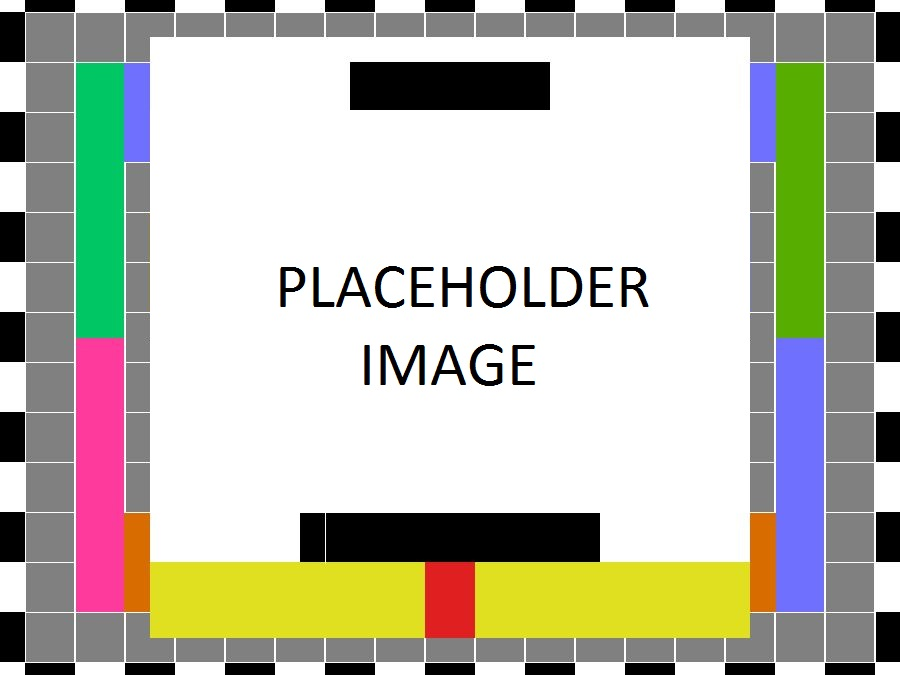
\includegraphics[width=0.60\textwidth]{images/test_image}
    \caption{X conceptual drawing}
\end{figure}

\newpage
\section{Product Description}
This section provides a description of your product and defines it's primary features and functions. The purpose is to give the document reader/reviewer enough information about the product to allow them to easily follow the specification of requirements found in the remainder of the document. Your header for this section should introduce the section with a brief statement such as: "This section provides the reader with an overview of X. The primary operational aspects of the product, from the perspective of end users, maintainers and administrators, are defined here. The key features and functions found in the product, as well as critical user interactions and user interfaces are described in detail." Using words, and pictures or graphics where possible, specify the following:

\subsection{Features \& Functions}
What the product does and does not do. Specify in words what it looks like, referring to a conceptual diagram/graphic (Figure X).  Define the principle parts/components of the product. Specify the elements in the diagram/graphic that are part(s) of this product as well as any associated external elements (e.g., the Internet, an external web server, a GPS satellite, etc.)

\subsection{External Inputs \& Outputs}
Describe critical external data flows. What does your product require/expect to receive from end users or external systems (inputs), and what is expected to be created by your product for consumption by end users or external systems (outputs)? In other words, specify here all data/information to flow into and out of your systems. A table works best here, with rows for each critical data element, and columns for name, description and use.

\subsection{Product Interfaces}
Specify what all operational (visible) interfaces look like to your end-user, administrator, maintainer, etc. Show sample/mocked-up screen shots, graphics of buttons, panels, etc. Refer to the critical external inputs and outputs described in the paragraph above.

\newpage
\section{Customer Requirements}
The nature of this product lends itself to creativity and flexibility in the requirements gathering process. Throughout the process, thought was given to the purpose and eventual use of the laser harp. Keeping in mind that the end users will be young middle school to high school students who are interested in STEM, we created the following Customer Requirements.
\subsection{Product shall use visible laser beams}
\subsubsection{Description}
The product shall use laser beams that, when broken/interrupted, will signal the device to produce a tone. An array of laser diodes will be arranged across the top of the device and shine down onto photo-resistors that will detect the breaks and relay that information to an onboard microcontroller. The beams shall be made visible through the use of a fogger that allows the laser beam to reflect and appear to shine.
\subsubsection{Source}
Customer: Dr. McMurrough
\subsubsection{Constraints}
We will be limited to the type and number of components that can be connected to a single microcontroller.
\subsubsection{Standards}
N/A
\subsubsection{Priority}
Critical

\subsection{Built-In Speakers}
\subsubsection{Description}
The product shall have speakers to generate the tones/sounds. These speakers shall be connected to the onboard software synthesizer that controls the sound generation and will be located on the base of the device.
\subsubsection{Source}
Development Team
\subsubsection{Constraints}
Space will be a constraint as the base will be of limited size.
\subsubsection{Standards}
N/A
\subsubsection{Priority}
Critical

\subsection{Polyphony}
\subsubsection{Description}
The onboard synthesizer shall have the ability to take the input of two or more laser beams at the same time and output the combined tone to play from the speakers.
\subsubsection{Source}
Development Team
\subsubsection{Constraints}
We will be limited by the capabilities of the software synthesizer we use, which will the maximum number of voices the synth allows.
\subsubsection{Standards}
N/A
\subsubsection{Priority}
High


\subsection{MIDI Device}
\subsubsection{Description}
The device shall have the ability to be used as a MIDI device. The device shall be able to connect via USB or a MIDI connector to a MIDI Synthesizer for sound generation. The output of the device shall be a serial MIDI signal.
\subsubsection{Source}
Customer: Dr. McMurrough
\subsubsection{Constraints}
We will be constrained by the existing protocol for serialized MIDI signals.
\subsubsection{Standards}
MIDI 1.0
\subsubsection{Priority}
High

\subsection{Ease of Use}
\subsubsection{Description}
The device shall be easy to play and generate sounds in an intuitive manner. Given that this product will be used for outreach and as a tool to keep kids interested in STEM, the product should be intuitive, quick to learn, and easy to use.
\subsubsection{Source}
Customer: Dr. McMurrough
\subsubsection{Constraints}
The ease of use will be evaluated with middle to high school students in mind. The device must not be too cumbersome or complex for the typical child in that age group.
\subsubsection{Standards}
N/A
\subsubsection{Priority}
High

\subsection{Portability}
\subsubsection{Description}
The product shall be portable for use in remote outreach events. The product shall be light enough to be carried by a single person. The product will be powered by a  power source to eliminate the need for an outlet. The product shall have a handle for ease of carrying.
\subsubsection{Source}
Development Team
\subsubsection{Constraints}
A max weight of 50 lbs must not be exceeded.
\subsubsection{Standards}
OSHA recommendations
\subsubsection{Priority}
Moderate

\subsection{Configurable}
\subsubsection{Description}
The device shall have the ability to be configured to adjust certain settings. Settings that must be configurable include: volume, pitch, attack, sustain, release, etc. These settings will be configured using controls on the base of the device.
\subsubsection{Source}
Customer: Dr. McMurrough
\subsubsection{Constraints}
Existing devices shall serve as guides for how and what can be configured.
\subsubsection{Standards}
N/A
\subsubsection{Priority}
Moderate

\subsection{Preset Instrument Sounds}
\subsubsection{Description}
The MIDI Synthesizer shall be preloaded with preset configurations to emulate certain instruments. Instruments to emulate include: Harp, Piano, Guitar, Flute, & more.
\subsubsection{Source}
Customer: Dr. McMurrough
\subsubsection{Constraints}
We must accurately simulate the instruments we select. A user must be able to tell which instrument is being played.
\subsubsection{Standards}
N/A
\subsubsection{Priority}
Moderate

\subsection{Visual Requirement}
\subsubsection{Description}
The device shall be visually appealing. The device shall not contain any exposed wiring and should have some sort of finish to look good.
\subsubsection{Source}
Development Team
\subsubsection{Constraints}
If the device is made of wood, the wood must be painted and varnished. Electronic components, other than controls and displays, must not be visible. Generally, the device should look like something you would want to use.
\subsubsection{Standards}
N/A
\subsubsection{Priority}
Moderate

\subsection{Audio Output & External Output}
\subsubsection{Description}
The device shall play audio internally and also offer external output options to play audio on external speakers.
\subsubsection{Source}
Development Team
\subsubsection{Constraints}
The output is constrained by the sound card capabilities and output options it has.
\subsubsection{Standards}
N/A
\subsubsection{Priority}
Critical

\subsection{Power and Volume}
\subsubsection{Description}
The device will have a volume slider to control the output gain.
\subsubsection{Source}
Development Team
\subsubsection{Constraints}
N/A
\subsubsection{Standards}
The device shall be able to run off a 12 V power supply.
\subsubsection{Priority}
Critical

\subsection{Design}
\subsubsection{Description}
The device shall look like a harp.
\subsubsection{Source}
Customer: Dr. McMurrough
\subsubsection{Constraints}
The design is constrained by what we can feasibly manufacture and 3D print.
\subsubsection{Standards}
N/A
\subsubsection{Priority}
Critical

\subsection{Design Robustness}
\subsubsection{Description}
The device shall stand upright without the need for external support.
\subsubsection{Source}
Development Team
\subsubsection{Constraints}
The device needs to be stable while also having a design that is aesthetically pleasing.
\subsubsection{Standards}
N/A
\subsubsection{Priority}
Moderate

\subsection{Mass}
\subsubsection{Description}
The device shall not weigh over 50 pounds.
\subsubsection{Source}
Development Team
\subsubsection{Constraints}
The device cannot be too heavy as it needs to be portable.
\subsubsection{Standards}
N/A
\subsubsection{Priority}
High

\subsection{Speakers & Controls}
\subsubsection{Description}
The device shall have the speakers and controls at the base of the base of the device.
\subsubsection{Source}
Development Team
\subsubsection{Constraints}
The base of the device is where the internals will be kept, which also has the most room for controls that affect the device.
\subsubsection{Standards}
N/A
\subsubsection{Priority}
High
\newpage
\section{Packaging Requirements}
Include a header paragraph here. Packaging requirements are those requirements that identify how the delivered product will be packaged for delivery to the end-user; or how it will "look" when finished and delivered. For example, you might specify that the software required for operation will be pre-loaded on the hard drive, delivered on CD/DVD, or available via download. Software might be customer installable, or not, etc. Hardware components could be all in a single package, provided as a "bag of parts" to be assembled/installed by the user, painted a certain color, logos affixed, etc. Care should be taken not to duplicate requirements found in other sections of this document.

\subsection{Requirement Name}
\subsubsection{Description}
Detailed requirement description...
\subsubsection{Source}
Source
\subsubsection{Constraints}
Detailed description of applicable constraints...
\subsubsection{Standards}
List of applicable standards
\subsubsection{Priority}
Priority
\newpage
\section{Performance Requirements}
In this section, the performance of the Laser Harp is evaluated. It is very crucial that the laser harp lives up to the standard, the customer expects it to. Response time, startup time, reliability, etc. are some of the factors that are being evaluated to define the performance of the product.

\subsection{The device shall have a maximum setup time of 5 minutes.}
\subsubsection{Description}
The time taken to set up the equipment should be less than 5 minutes. The process includes wiring the necessary components, aligning the laser diodes to photoresistors if not already done, and connecting to power source.
\subsubsection{Source}
Team
\subsubsection{Constraints}
Most of the components should already be wired and in position i.e. no breadboard connections required and laser diodes and photoresistors should be already on the frame, so that not a lot work is needed to align the parts in the correct place. There must be an appropriate power source nearby.
\subsubsection{Standards}
N/A
\subsubsection{Priority}
Medium

\subsection{The device shall startup and fully boot within 30 seconds.}
\subsubsection{Description}
Once the all the components of the device are setup, the device should take no longer than 30 seconds to be fully operational. Users should be able to see the lasers and play sound by interfering the laser beams.
\subsubsection{Source}
Team
\subsubsection{Constraints}
All components should be in place and the laser diodes should be pointed towards the photoresistors.
\subsubsection{Standards}
N/A
\subsubsection{Priority}
Medium

\subsection{The device shall be able to play audio to stereo.}
\subsubsection{Description}
The audio output should be able to be redirected towards stereo. Instead of piezo speaker, the audio should come out of stereo without any difficulty.
\subsubsection{Source}
Team
\subsubsection{Constraints}
The device should be fully operational and necessary outputs must be visible.
\subsubsection{Standards}
N/A
\subsubsection{Priority}
Low

\subsection{The device should have very low latency between the laser being triggered and resulting audio playback.}
\subsubsection{Description}
Once the laser beam is interfered, there should be no or minimal delay in the resulting audio. The sound should vary with respect to the laser that is being triggered. The time taken to hear audio should be less than 100 milliseconds.
\subsubsection{Source}
Team
\subsubsection{Constraints}
The device should be fully operational, and it should be connected to necessary audio output. No other devices should be playing nearby.
\subsubsection{Standards}
N/A
\subsubsection{Priority}
High

\subsection{The device should be reliable and should not crash during use.}
\subsubsection{Description}
The device should not crash or turn off by itself unless the power source is removed. If adequate power supply is provided and all the parts not corroded, the device should run for few hours without crashing. 
\subsubsection{Source}
Team
\subsubsection{Constraints}
All the parts should be in good condition. All the connection should be tight and insulated from any external factors. There should be a constant power source.
\subsubsection{Standards}
IEEE 1413.1-2002
\subsubsection{Priority}
High

\newpage
\section{Safety Requirements}
The laser harp project deals with lasers which can damage the eyes and be hazardous if we are not careful. There are also wires, mister, speakers and power source that is needed to be handled carefully.

\subsection{The lasers on the device should be put in a way they do not point towards anyone’s eyes}
\subsubsection{Description}
The lasers mounted on the product should be fixed and immovable. It should in no way be pointed anywhere else but the receiving sensors. It should not diverge from the path at any angle.
\subsubsection{Source}
CSE Senior Design laboratory policy
\subsubsection{Constraints}
The laser pointers will be made immovable and fixed to a certain place to minimize risks and will be in compliance with the ANSI Z136 standards.
\subsubsection{Standards}
ANSI Z136.1 – Safe use of lasers
\subsubsection{Priority}
Critical

\subsection{The laser should only point to the receiving sensor.}
\subsubsection{Description}
The lasers should in no way be pointed anywhere else but the receiving sensors. It should be a straight path from the laser pointer to the sensors.
\subsubsection{Source}
CSE Senior Design laboratory policy
\subsubsection{Constraints}
The lasers will be in compliance with the ANSI Z136 standards.
\subsubsection{Standards}
ANSI Z136.1 – Safe use of lasers
\subsubsection{Priority}
Critical

\subsection{The device and all the internal parts should be enclosed.}
\subsubsection{Description}
The internal components i.e. Arduino, speakers, wires, etc. should all be enclosed in a main box/frame so that they are protected from the outside interference.
\subsubsection{Source}
CSE Senior Design laboratory policy
\subsubsection{Constraints}
The external structure will not be authorized to be taken apart by anyone except the instructor and project members.
\subsubsection{Standards}
Occupational Safety and Health Standards
\subsubsection{Priority}
Critical

\subsection{The mister should not damage any internal components.}
\subsubsection{Description}
The mister should be on the outside part of the product and should not affect/harm any internal components.
\subsubsection{Source}
CSE Senior Design laboratory policy
\subsubsection{Constraints}
mister will only be used only when needed in limited amount by authorized personnel.
\subsubsection{Standards}
Occupational Safety and Health Standards
\subsubsection{Priority}
Critical

\subsection{The mister should not cause health problems.}
\subsubsection{Description}
The mister should be safe to use and should not cause any health problems to anyone.
\subsubsection{Source}
CSE Senior Design laboratory policy
\subsubsection{Constraints}
mister will only be used only when needed in limited amount by authorized personnel.
\subsubsection{Standards}
Occupational Safety and Health Standards
\subsubsection{Priority}
Critical

\subsection{The external wires should be properly insulated on the device.}
\subsubsection{Description}
All of the wires should be properly insulated. They should be in compliance with all the requirements specified in the National Electric Code.
\subsubsection{Source}
CSE Senior Design laboratory policy
\subsubsection{Constraints}
High voltage power sources, as defined in NFPA 70, will be avoided as much as possible in order to minimize potential hazards.
\subsubsection{Standards}
NFPA 70
\subsubsection{Priority}
Critical

\subsection{The physical device shall be structurally firm about its base.}
\subsubsection{Description}
The whole product should be firm and stable upright. It should not be able to be easily tipped when upright. It should also be sturdy enough.
\subsubsection{Source}
CSE Senior Design laboratory policy
\subsubsection{Constraints}
The device will only be used by team members and the professor.
\subsubsection{Standards}
Occupational Safety and Health Standards
\subsubsection{Priority}
Critical

\newpage
\section{Maintenance \& Support Requirements}
Include a header paragraph specific to your product here. Maintenance and support requirements address items specific to the ongoing maintenance and support of your product after delivery. Think of these requirements as if you were the ones who would be responsible for caring for customers/end user after the product is delivered in its final form and in use "in the field". What would you require to do this job? Specify items such as: where, how and who must be able to maintain the product to correct errors, hardware failures, etc.; required support/troubleshooting manuals/guides; availability/documentation of source code; related technical documentation that must be available for maintainers; specific/unique tools required for maintenance; specific software/environment required for maintenance; etc.

\subsection{Requirement Name}
\subsubsection{Description}
Detailed requirement description...
\subsubsection{Source}
Source
\subsubsection{Constraints}
Detailed description of applicable constraints...
\subsubsection{Standards}
List of applicable standards
\subsubsection{Priority}
Priority
\newpage
\section{Other Requirements}
Include a header paragraph specific to your product here. In this section specify anything else that is required for the product to be deemed complete. Include requirements related to customer setup and configuration if not specified in a previous requirement. Add any known requirements related to product architecture/design, such as modularity, extensibility (for future enhancements), or adaptation for a specific programming language. Consider requirements such as portability of your source code to various platforms (Windows, Linux, Unix Mac OS, etc.).

\subsection{Requirement Name}
\subsubsection{Description}
Detailed requirement description...
\subsubsection{Source}
Source
\subsubsection{Constraints}
Detailed description of applicable constraints...
\subsubsection{Standards}
List of applicable standards
\subsubsection{Priority}
Priority
\newpage
\section{Future Items}
In this last section, you will reiterate all requirements that are listed as priority 5. This is repetitive, but necessary as a concise statement of features/functions that were considered/discussed and documented herein, but will NOT be addressed in the prototype version of the product due to constraints of budget, time, skills, technology, feasibility analysis, etc. Use the following format for this section.
Our future requirements mostly be software enhancements that will improve the experience of the user when using the system. These requirements will be addressed once all other requirements have been met. 

\subsection{Loading Presets from Mobile Application}
\subsubsection{Description}
The device should be able to play user presets within 5 seconds of uploading in the app.
\subsubsection{Source}
Development Team
\subsubsection{Constraints}
The user must be within close proximity of the device. The user must also be able to connect via bluetooth to the device. 
\subsubsection{Standards}
802.11 Bluetooth protocol.
\subsubsection{Priority}
Future

\subsection{Time of Flight Sensors}
\subsubsection{Description}
The system shall use time of flight sensors to adjust output of sound.
\subsubsection{Source}
Development Team
\subsubsection{Constraints}
Time of flight sensors are typically invisible to finding one with visible light will be difficult. 
\subsubsection{Standards}
N/A
\subsubsection{Priority}
Future

\subsection{Bluetooth Connectivity}
\subsubsection{Description}
The system shall be able to connect to Bluetooth speakers for audio output.
\subsubsection{Source}
Development Team
\subsubsection{Constraints}
Speakers must be within close proximity to the device or phone device.
\subsubsection{Standards}
802.11 Bluetooth protocol
\subsubsection{Priority}
Future

\subsection{User Sounds}
\subsubsection{Description}
The application shall be able to upload sound files to device.
\subsubsection{Source}
Development Team
\subsubsection{Constraints}
The system shall be able to intake sound files from the mobile application and play those sounds. The system must have sufficient capacity to store these sound files.
\subsubsection{Standards}
802.11 Bluetooth protocol
\subsubsection{Priority}
Future

\subsection{Configurability from Mobile application}
\subsubsection{Description}
Mobile app will be used to configure the device and expand functionality.
\subsubsection{Source}
Development Team
\subsubsection{Constraints}
The system will require a configuration file. Assume that Bluetooth is lossless and all packets get delivered.
\subsubsection{Standards}
802.11 Bluetooth protocol
\subsubsection{Priority}
Future

\subsection{Individual Laser Control}
\subsubsection{Description}
Individual lasers shall be able to be turned off and on based on preset
\subsubsection{Source}
Development Team
\subsubsection{Constraints}
The circuit must work without loss to cut power to laser. 
\subsubsection{Standards}
N/A
\subsubsection{Priority}
Future

\subsection{Physical Control Mechanisms for Sounds}
\subsubsection{Description}
The product shall have physical controls for: Attack, Decay, Sustain, Release, Volume, High-pass/Low-pass filters.
\subsubsection{Source}
Development Team
\subsubsection{Constraints}
The physical controls will eventually weardown. 
\subsubsection{Standards}
N/A
\subsubsection{Priority}
Future

\subsection{Preset Display}
\subsubsection{Description}
Presets for the instrument will be configured on the device using a button/knob and displayed on the screen
\subsubsection{Source}
Development Team
\subsubsection{Constraints}
The display will need to be dynamic (capable of switching images). Assume that display is powered with same power source as laser.
\subsubsection{Standards}
N/A
\subsubsection{Priority}
Future

\subsection{Custom Preset}
\subsubsection{Description}
On custom preset the device shall display "custom".
\subsubsection{Source}
Development Team
\subsubsection{Constraints}
The display must be large enough to display the word custom.
\subsubsection{Standards}
N/A
\subsubsection{Priority}
Future
\newpage

%%% References
\bibliographystyle{plain}
\bibliographystyle{reference/IEEEtran_custom}
\bibliography{reference/refs}{}

\end{document}
